% Scalar instruction entry source: tools/generate_scalar_instruction_catalog.py.
\subsection{\texttt{LSRGET}}
\label{sec:scalar-lsrget}
\index{LSRGET@\texttt{LSRGET}}
\begin{sloppypar}\noindent\textbf{Purpose.} Reads a system register identified by the ID operand and writes the value to the selected destination.\end{sloppypar}\smallskip
\noindent\textbf{Syntax.}\par
\begin{lstlisting}[style=ptoscalarcode]
lsrget LSR_ID, ->RegDst
\end{lstlisting}
\noindent\textbf{Encoding.}\par
\noindent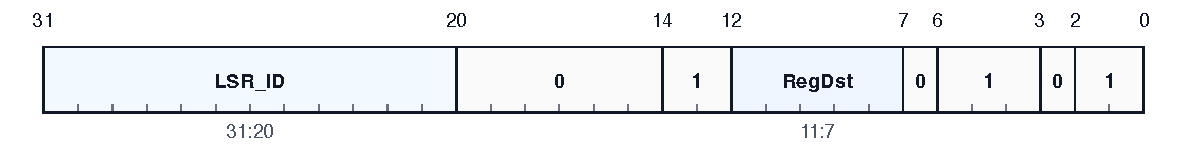
\includegraphics[width=\textwidth]{figs/encoding/scalar_instruction_entries/enc_lsrget.pdf}\par\smallskip
\begin{description}[leftmargin=0.18\linewidth,style=nextline]
\item[Format] \texttt{L32} \texttt{32-bit} scalar word.
\item[Pattern] \texttt{............00000011.....0111011}.
\end{description}
\noindent\textbf{Classification.}\par
\begin{description}[leftmargin=0.18\linewidth,style=nextline]
\item[Category] System, Cache, SSR, and Execution Control.
\item[Family] SSR Access.
\item[Execution class] \texttt{SYS}; uop\_kind=SYS, sys\_kind=SSR.
\end{description}
\noindent\textbf{Operand fields.}\par
\begin{description}[leftmargin=0.18\linewidth,style=nextline]
\item[\texttt{LSR\_ID}] Bits \texttt{31:20 (12b)}. 12-bit local/system register identifier selected by this register-access instruction.
\item[\texttt{RegDst}] Bits \texttt{11:7 (5b)}. 5-bit scalar destination register that receives the loaded value after any sign or zero extension; X0 discards the load result.
\end{description}
\noindent\textbf{Operation.}\par
\begin{lstlisting}[style=ptoscalarcode]
value = ReadSystemRegister(ID)
Write(RegDst, value)
\end{lstlisting}
\Needspace{0.08\textheight}
